\chapter{Implementierung}

\section{Scanner Konstruktion}
\label{sec:scannerKonstruktion}
Um das Lichtschnittverfahren angemessen umsetzen zu können, müssen zuerst brauchbare Daten erhoben werden. Mit Daten sind in diesem Kontext die Fotografien gemeint, auf denen das zu vermessende Objekt inklusive der projizierten Laserlinie zu sehen ist. Um diese Reihe von Bildern zu erstellen, ist eine Vorrichtung von Nöten, die es ermöglicht, die Webcam und den Laser so zu fixieren, dass das zu vermessene Objekt mit Leichtigkeit fotografierbar ist. Zusätzlich müssen sowohl der Laser als auch die Kamera so beweglich sein, dass das zu vermessene Objekt in kontrollierten Abständen mit dem Laser abgetastet werden kann, sich das räumliche Verhältnis zwischen Webcam und Laser sich jedoch nicht verändert. 

Für das vorliegende Projekt wurde versucht, dies unter Berücksichtigung einer einfachen und günstigen Konstruktion zu realisieren. Die in dieser Ausarbeitung vorgeschlagene Lösung setzt darauf, Kamera und Laser übereinander auf einer Pappelholzplatte zu fixieren. Diese Holzplatte befindet sich auf zum Boden senkrecht befindlichen Schlaufen aus stabilem Gurt, welche um zwei PVC-Röhren gespannt sind. Besagte PVC-Röhren ruhen in horizontaler Lage parallel zum Boden in zwei Holzstreben, welche wiederrum senkrecht auf einer Basis aus dünnem Pappelholz geklebt sind. Die Gesamtkonstruktion kann in Abb. \ref{fig:scanner1} und \ref{fig:scanner2} und betrachtet werden.

\begin{figure}
\centering
\begin{minipage}{0.45\textwidth}
\centering 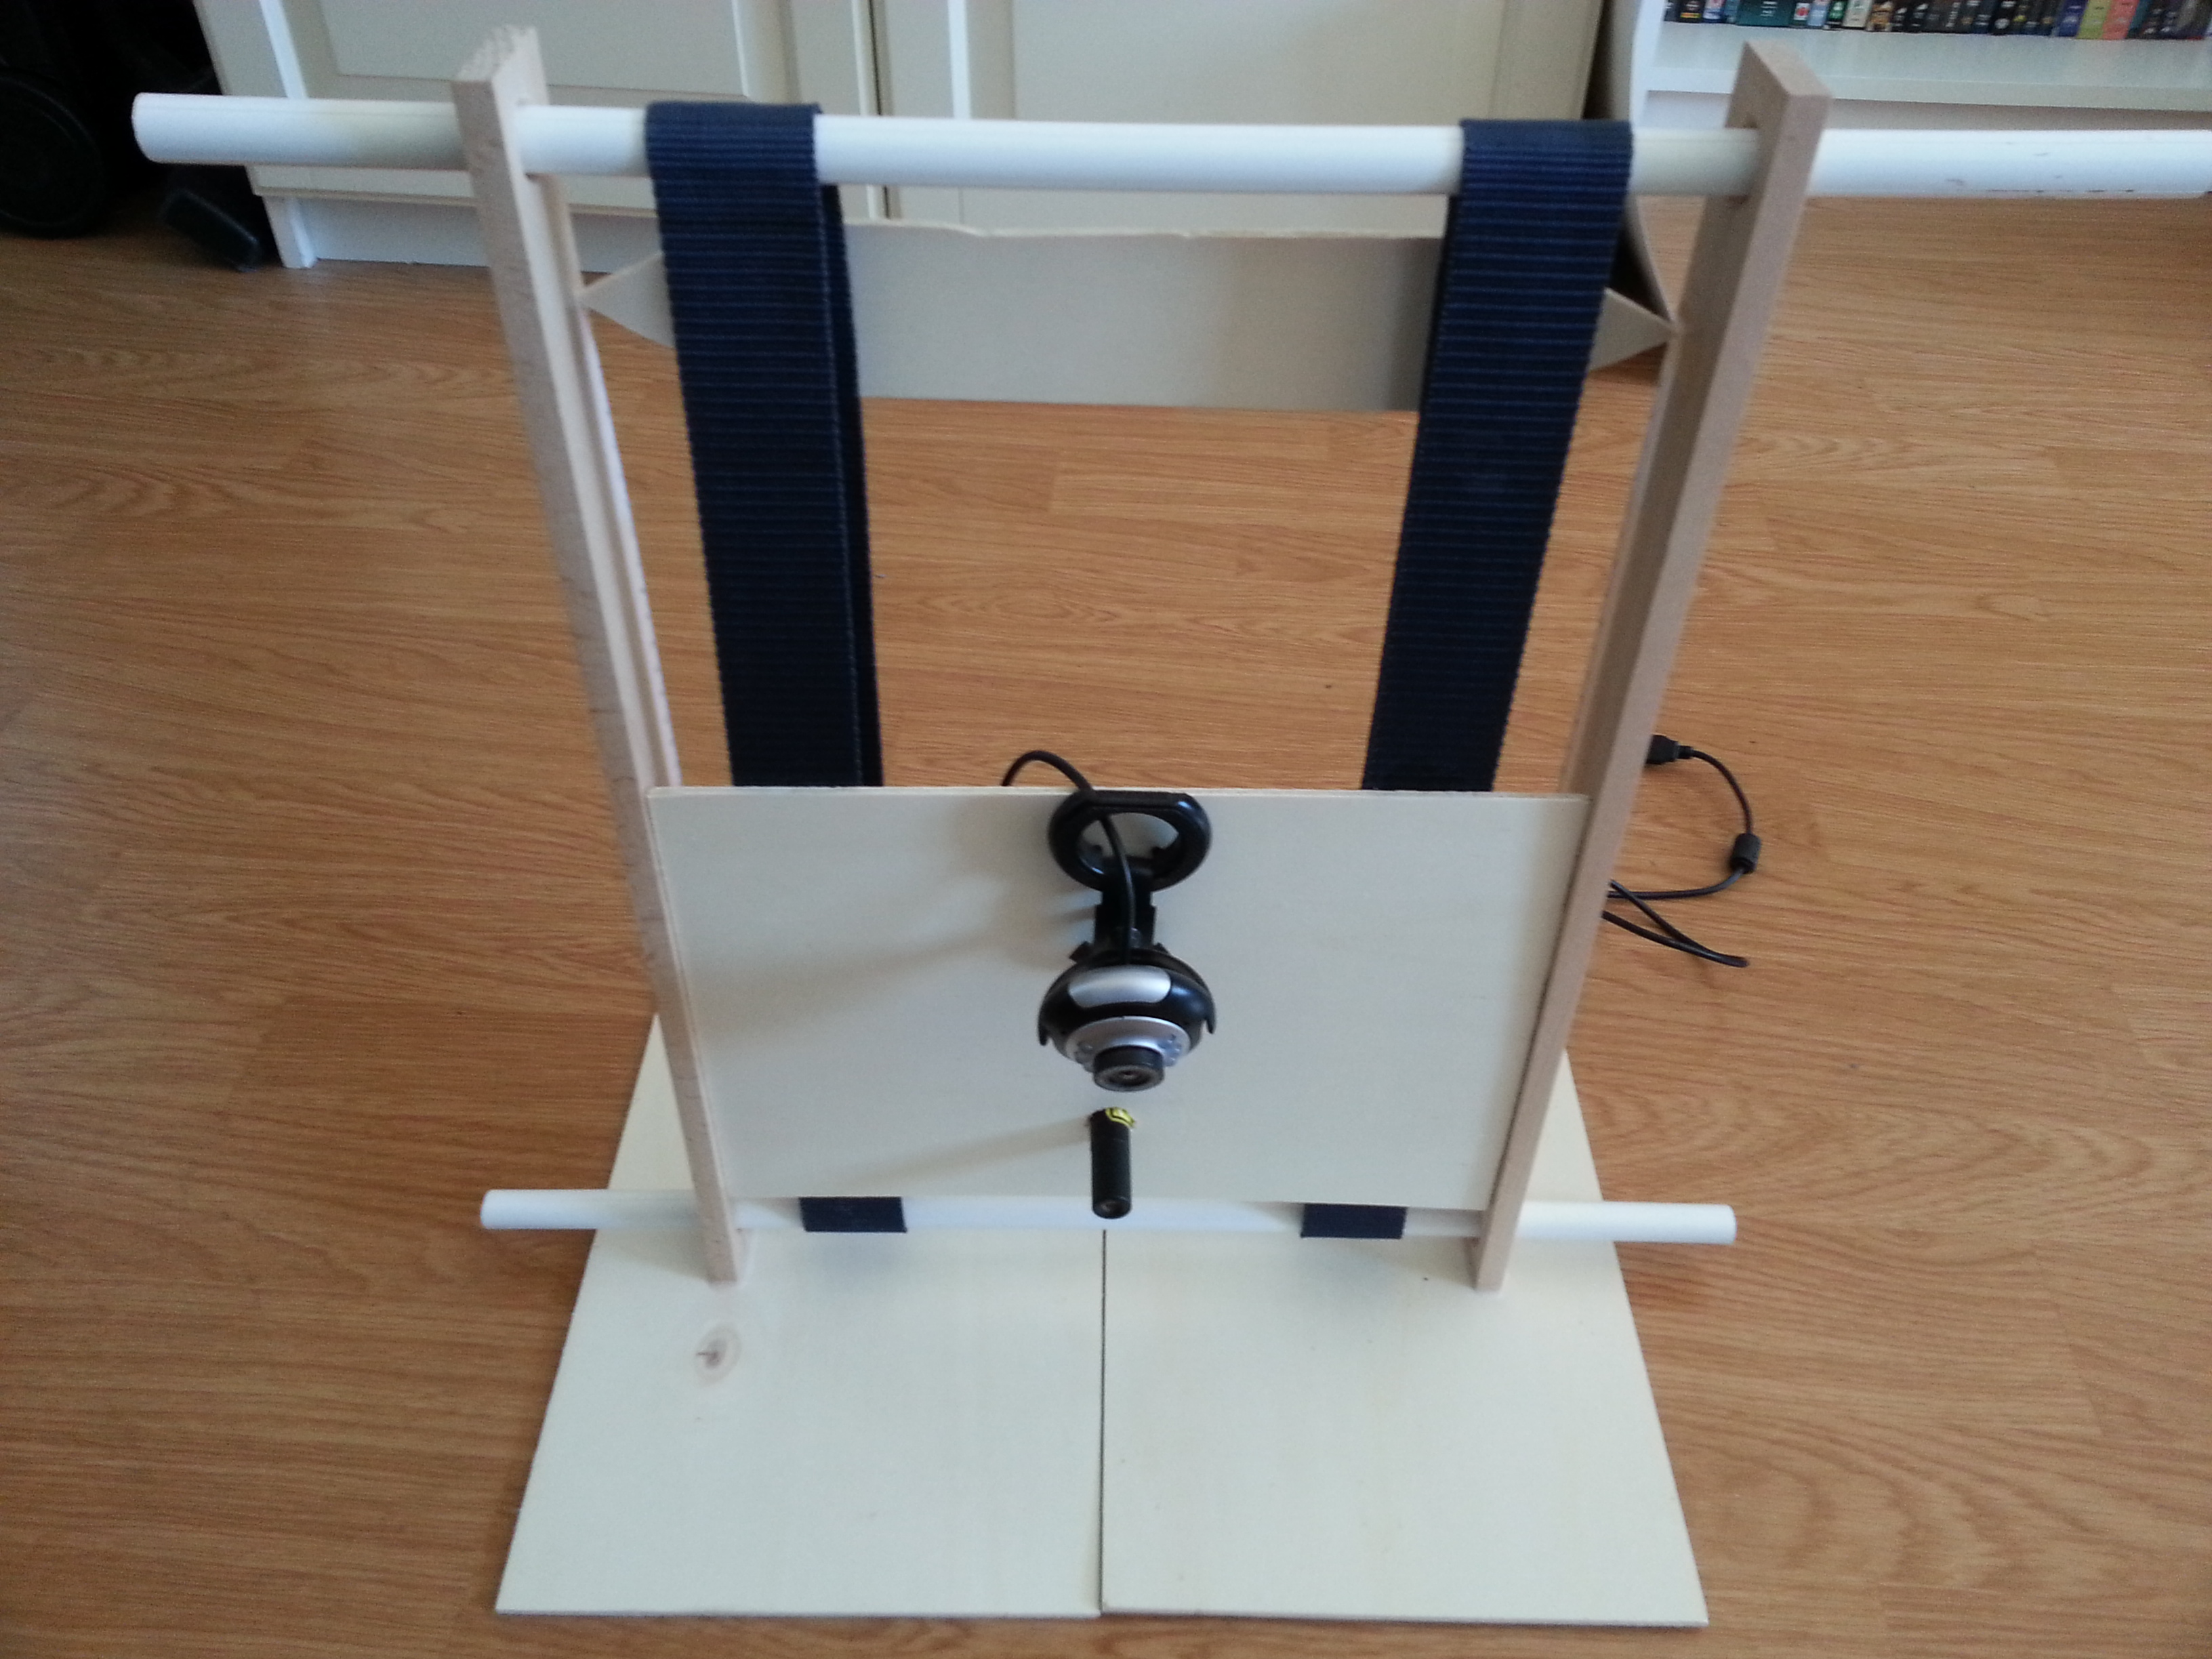
\includegraphics[width=\textwidth]{images/Scanner1.jpg}
\label{fig:scanner1}
\caption{Frontal Ansicht}
\end{minipage}
\begin{minipage}{0.45\textwidth}
\centering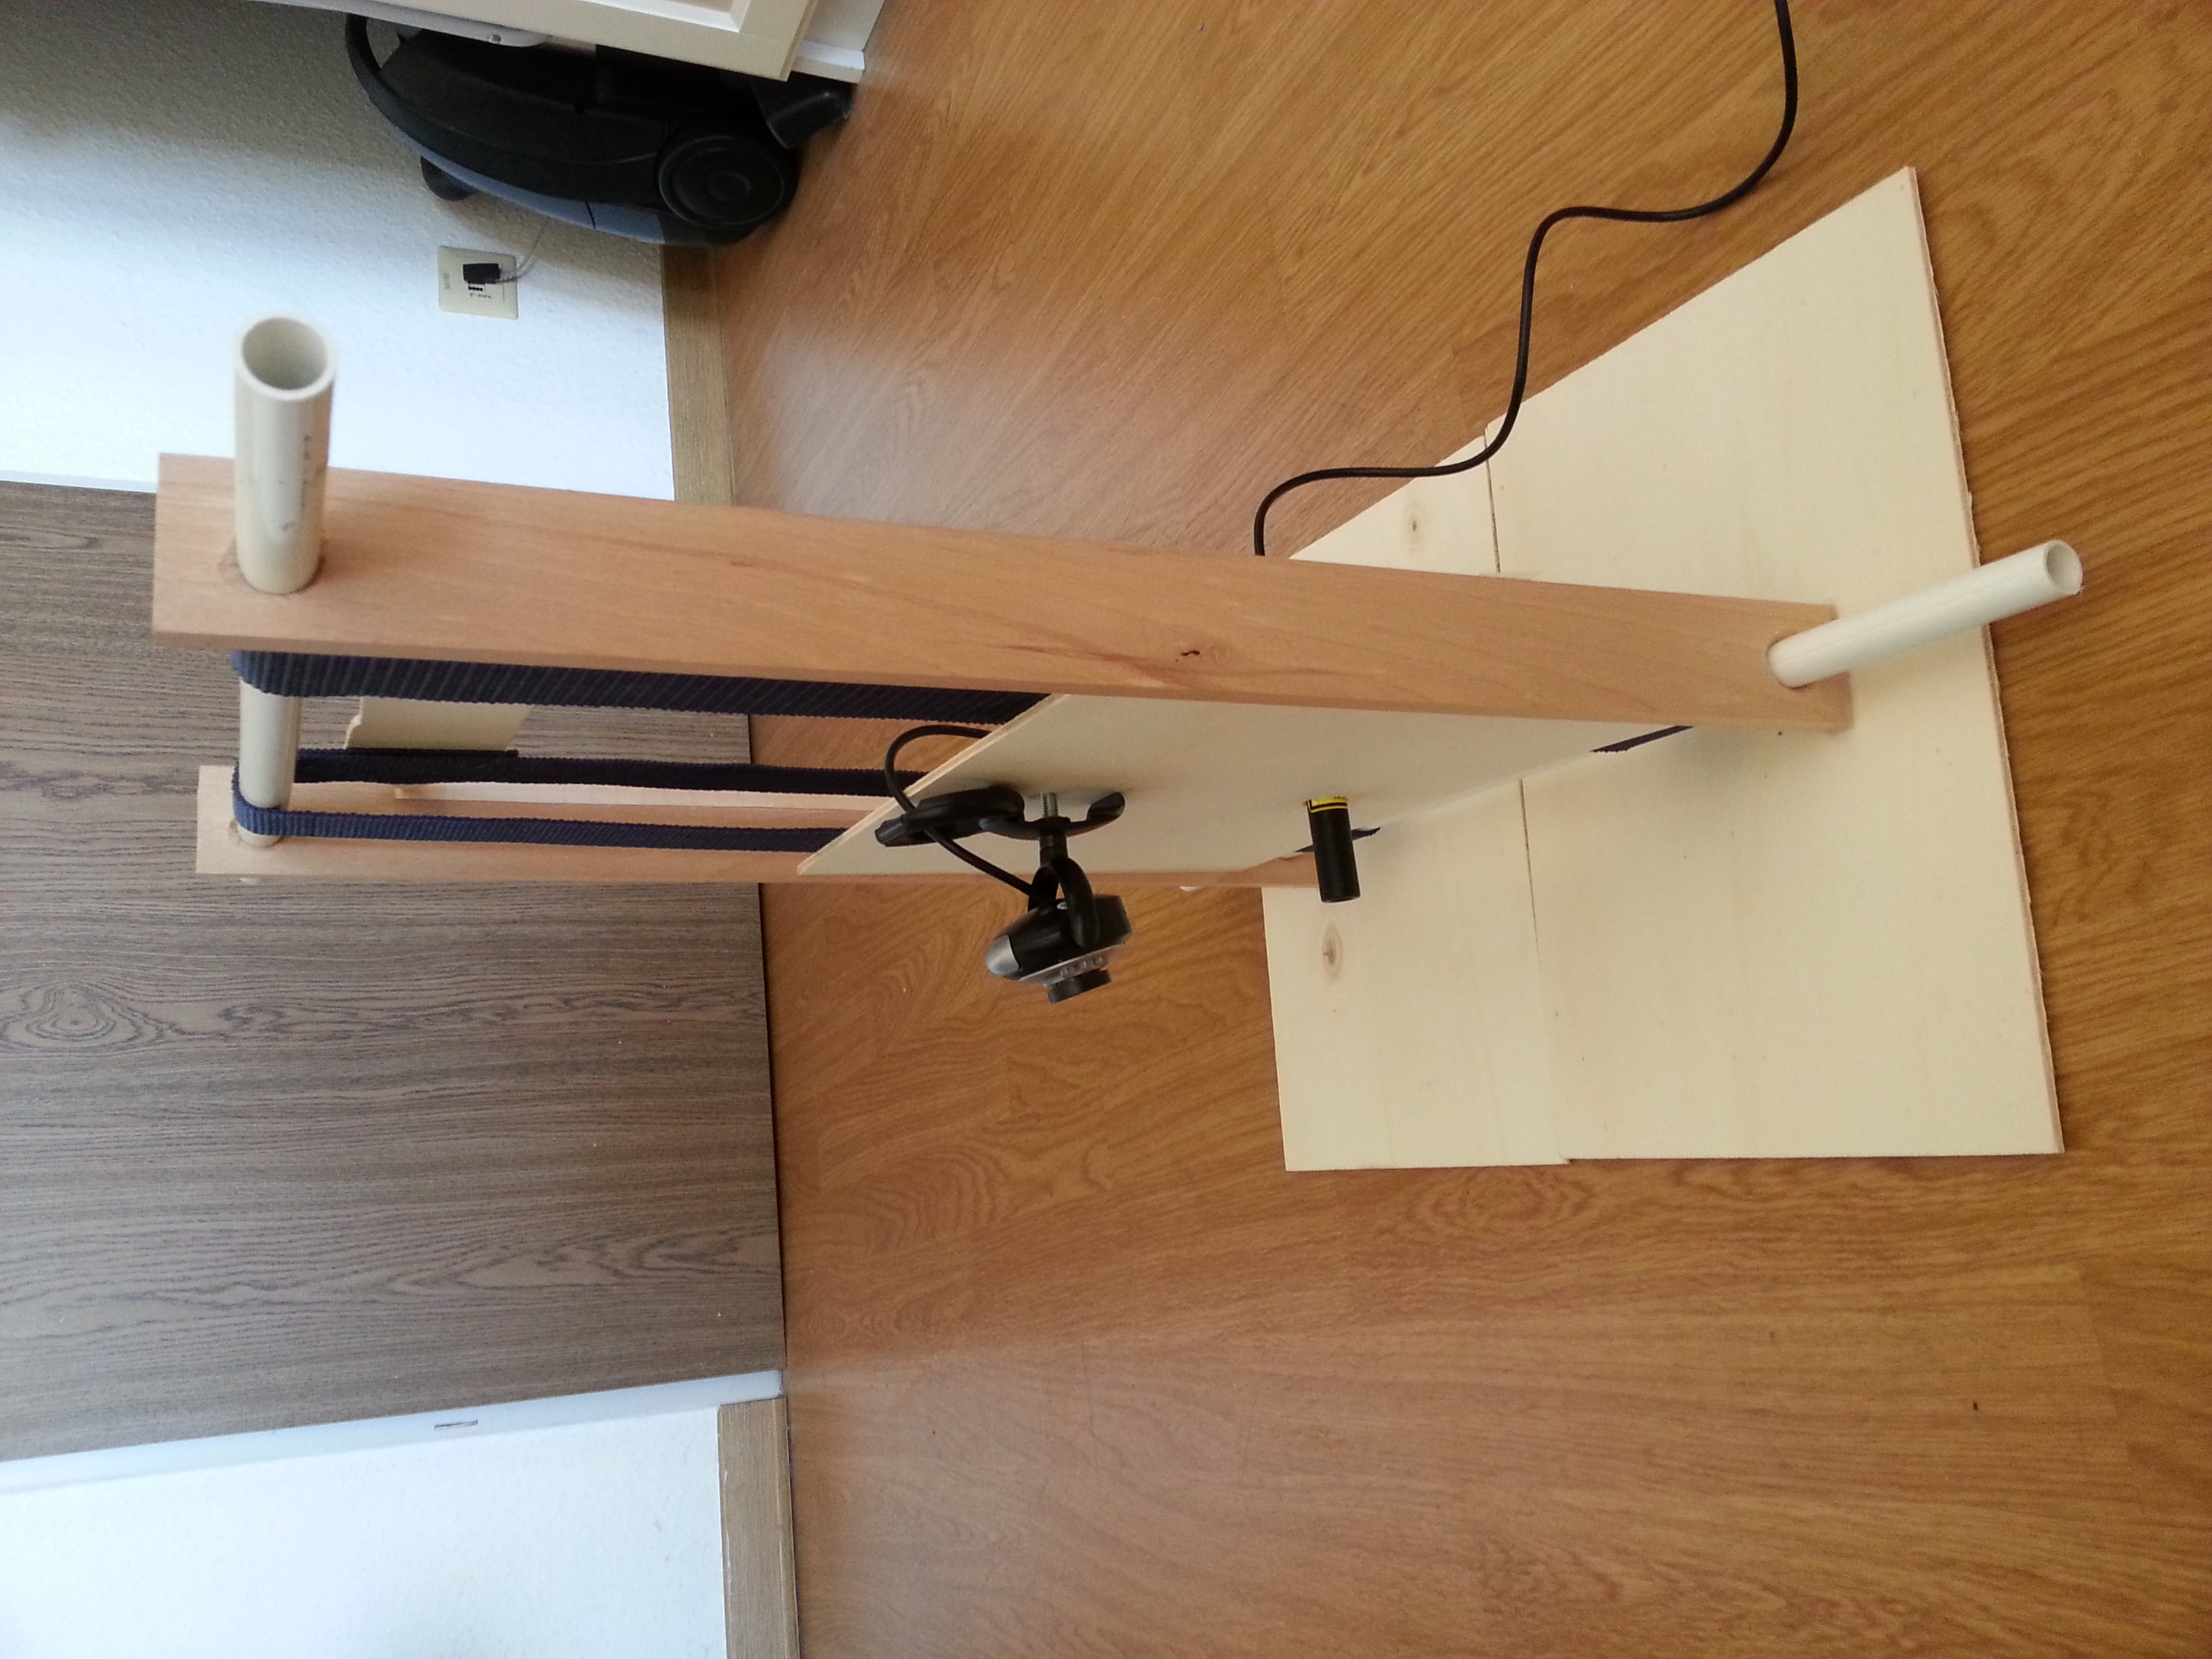
\includegraphics[width=\textwidth, angle = -90]{images/Scanner2.jpg}
\label{fig:scanner2}
\caption{Seitliche Ansicht}
\end{minipage}
\end{figure}

\begin{figure}
\centering 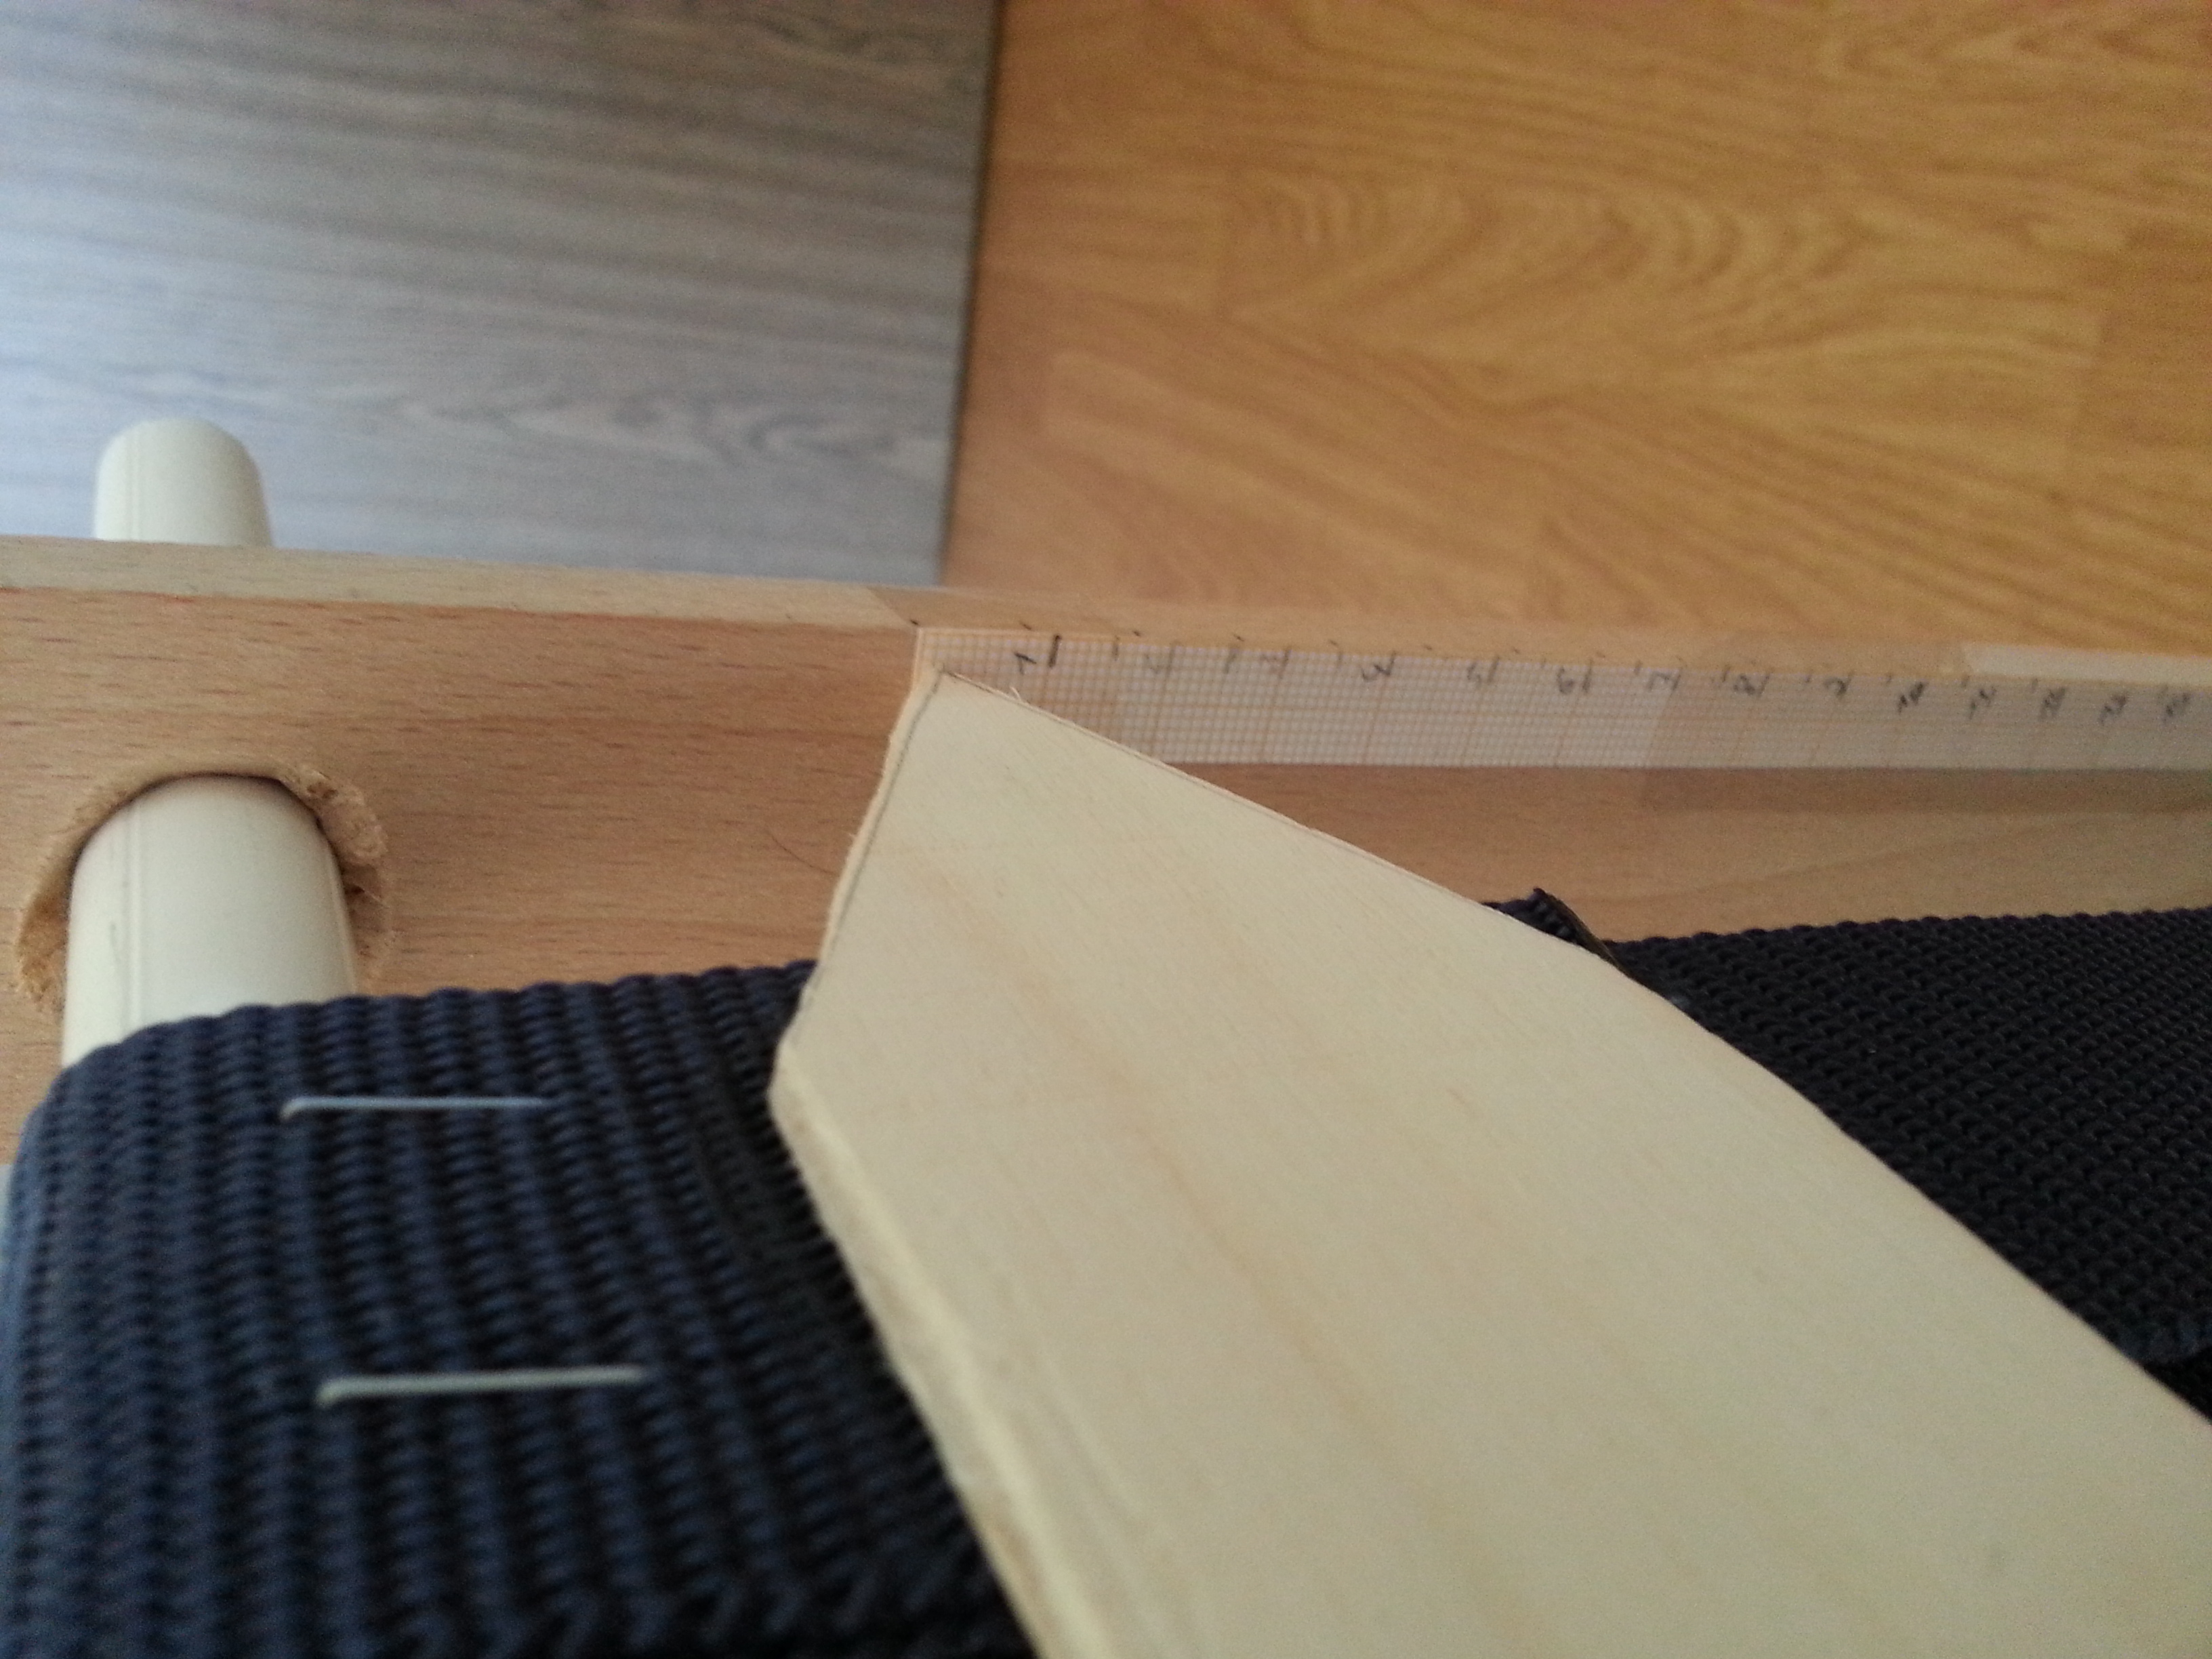
\includegraphics[width=0.5\textwidth, angle = -90]{images/Scanner3.jpg}
\label{fig:scanner3}
\caption{Nahaufnahme der Millimeter-Anzeige}
\end{figure}

Die vom Laser aufgespannte Ebene befindet sich somit parallel zum Grund, während die Kamera schräg von oben auf das zu vermessene Objekt schaut. Mittels des Gurts kann die Holzplatte, auf der Kamera und Laser montiert sind, von unten nach oben bewegt werden, um das Objekt so abzutasten. Um zu kontrollieren, wie weit der Laser über das Objekt bewegt wurde, ist auf der Rückseite des Gurts eine Anzeige installiert, welche sich gen Boden bewegt sobald Laser und Kamera nach oben steigen. Die Anzeige zeigt an den Seiten der Holzstreben, an denen eine Skala in Millieter-Papier angebracht ist, wie weit sich die Holzplatte von der Startposition aus nach oben bewegt hat. In Abb. \ref{fig:scanner3} ist eine Nahaufnahme dieser Anzeige zu sehen.

Ein wesentlicher Vorteil der vorgenommenen Konstruktion liegt in der Parallelität der Laser-Ebene zum Boden. Auf diese Weise muss man sich bei der späteren Bildverarbeitung keine Sorgen machen, dass die Laser-Linie auf den Untergrund fällt, auf dem das zu vermessene Objekt ruht. Wäre dies der Fall, müssten bei der späteren Auslesung die Teile der Laser-Linie, die auf das Objekt fallen, von denen, die auf den Untergrund fallen, aufwendig getrennt werden. Ebenfalls macht der Aufbau die Nachbearbeitung der gemessenen Weltkoordinaten im Gegensatz zu vergleichbaren Konstruktionen (z.B. bei schwenkbaren Scannern) besonders simpel: Da sich die Apparatur zwischen Aufnahmen lediglich entlang der Z-Achse bewegt und dieser Abstand bekannt ist, kann auf den Z-Achsen-Anteil des Messungsendergebnis der besagte Abstand einfach addiert werden.

Der Gesamtaufbau setzt vor allem auf eine praktikable Lösung, die problemlos nachgebaut werden kann und sich dem zu Grunde liegenden Problem so nähert, dass anschließende Verarbeitungen und Berechnungen erleichtert werden. Zudem ist die Konstruktion kostengünstig. In Tabelle \ref{tab:preise} können die Preise in Euro eingesehen werden, die alle Komponenten (außer Kleinteile wie einzelne Schrauben, Holzleim etc.) gekostet haben. Zusammen kommt der Scanner auf einen Preis von ca. 45,14\euro

\begin{table} %[hbtp]
	\centering
		\begin{tabular}{l | l}
		\textbf{Komponente} & \textbf{Preis in Euro}\\
		\hline
			Kamera "`TeckNet C016 USB HD Webcam"' & 13,99 \euro\\
			Linienlaser &  ca. 20 \euro\\
			PVC-Röhre & 1,69 \euro\\
			Holzleiste Buche (Seitenstreben) & 3,79 \euro\\
			Pappel-Sperrholz &  2,29 \euro\\
			Gurtband & 3,38 \euro
		\end{tabular}
	\caption{Bezeichnung der Tabelle}
	\label{tab:preise}
\end{table}


\section{Der Scanvorgang}
\label{sec:scanvorgang}
Um ein zu vermessendes Objekt in eine Reihe von abgetasteten Weltkoordinaten umzuwandeln wird in der vorliegenden Implementierung ein Prozess von verschiedenen Stufen vorgeschlagen. Der Gesamtprozess ist schematisch in Abb. \ref{fig:scanVorgang} dargestellt. Die einzelnen Stufen des Prozesses sind dabei nach der Abhängigkeit ihrer Ergebnisse und daraus folgen der Anzahl an nötigen Wiederholungen sortiert. Mit anderen Worten: Die Aktionen, die nur nur einmal ausgeführt werden müssen um mehrere Scanvorgänge zu ausführen zu können werden zuerst vorgenommen, während Aktionen die beispielsweise pro aufgenommenen Bild ausgeführt werden müssen, am Schluss folgen. Dies ist für denjenigen, der den Scanvorgang durchführt, eine geeignete Reihenfolge, da so Teilergebnisse für mehrere Scanprozesse wiederverwendet werden können und bei erfolglosen Stufen der Gesamtprozess nicht von neu angestoßen werden muss. \newline
Die Kalibrierung der internen Kameraparameter beispielsweise ist unabhängig von den anderen Umständen des eigentlichen Scanvorgangs und muss nicht für jede Messreihe erneut stattfinden, sondern lediglich wenn sich die Fokus-Einstellung der Kamera ändert. In der darauf folgenden Stufe des Scannens werden die nötigen Fotografien aufgenommen, was im Folgenden als Datenerhebung bezeichnet wird. Anschließend werden anhand einiger weniger dieser Bilder weitere Kalibrierungen vorgenommen, welche allerdings für den Rest des Datensatzes persistent sind und nur von Scandurchlauf zu Scandurchlauf wiederholt werden müssen. Zuletzt werden auf allen Bildern des Datensatzes die beiden Schritte der Laserlinienerkennung und Weltkoordinatenberechnung ausgeführt, welche für jedes Bild des Datensatzes andere Ergebnisse liefern und damit am Ende der Pipeline stehen. Die Weltkoordinaten, die als Resultat eines jeden Bildes berechnet werden, werden gesammelt und stehen als Punkte-Wolke zu weiteren Verarbeitung zur Verfügung. Im Folgenden werden nun die einzelnen Stufen des Scanvorgangs einzeln näher erläutert.


\begin{wrapfigure}{L}{0.45\textwidth}
\centering 
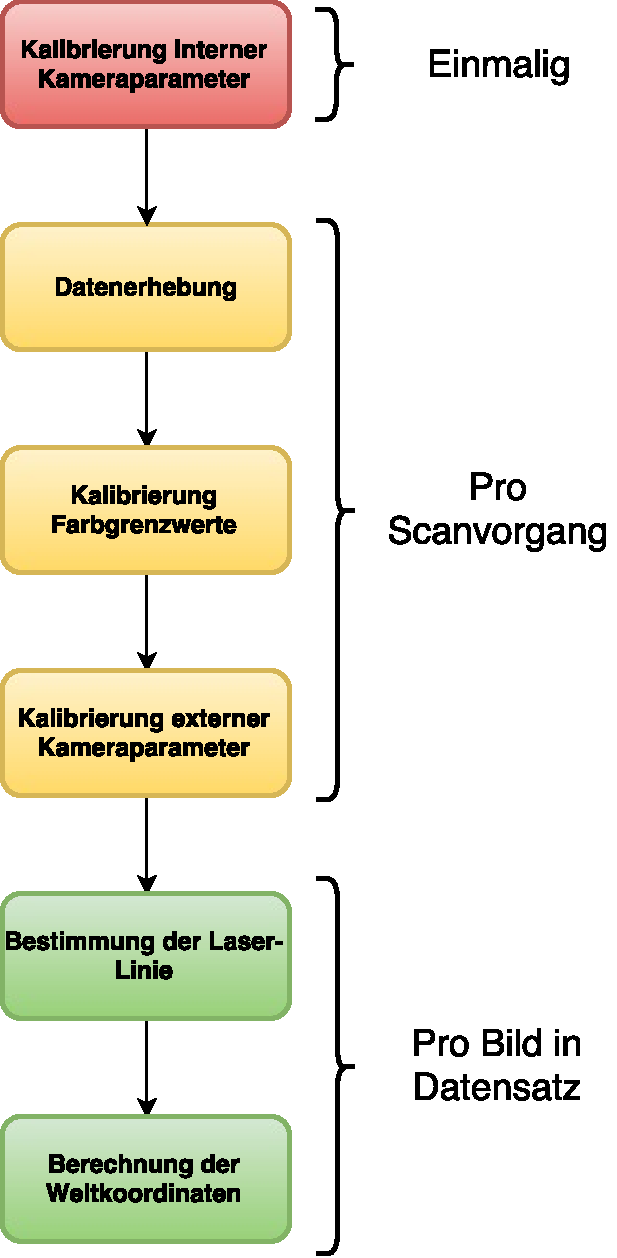
\includegraphics[width=0.45\textwidth]{images/ScannerVerfahren.pdf}
\label{fig:scanVorgang}
\caption{Der schematische Ablauf des Scanvorgangs}
\end{wrapfigure}
\leavevmode

\subsection{Kalibrierung der internen Kameraparameter}
In Abschnitt \ref{subsec:KameraKalibrierungTheorie} wurde die Theorie hinter der Kamerakalibrierung bereits erläutert, daher soll das Verfahren an dieser Stelle lediglich aus praktischer Sicht betrachtet werden. Aus Gründen, welche in \ref{fig:scanVorgang} dargelegt wurden, ist der Kamerakalibreirungsprozess in zwei zeitlich voneinander getrennte Teile gespalten. Am Anfang steht hierbei die Bestimmung der internen Kameraparamtern, insbesondere der internen Kameramatrix. Um diese abzuschätzen wurde auf die in Matlab integrierte Kamerakalibrirungsapp zurückgegriffen, welche aus einem Set von vorher aufgenommenen Bildern die Kameraparameter (wie in \ref{subsec:KameraKalibrierungTheorie} beschrieben) schätzt. Dabei werden eine Reihe von Kalibrierungsbilder, welche vorher aufgenommen wurden, in die App importiert und anschließend von jener verarbeitet. Bevor die nun geschätzte interne Kameramatrix als eigenständige Datei exportiert werden kann, sollten die sogenannten Reprojection Errors begutachtet werden. Diese stellen eine Metrik dar, welche besagt wie erfolgreich die Kalibrierung verlaufen ist und ergibt sich aus dem Abstand zwischen den im Bild erkannten Schachbrett-Punkten und den auf das Bild zurück projizierten korrespondierenden Weltkoordinaten (mehr dazu auch bei !QUELLE! und !QUELLE!). Bei den dieser Ausarbeitung mitgelieferten Kalibrierungsbilder wurde ein durchschnittlicher Reprojection Error von !WERT! erreicht, jedoch gilt laut einer Faustregel aus !QUELLE! jeder durchschnittliche Fehler von unter einem Pixel als akzeptabel. Am Ende der Kalibrierung muss die interne Kameramatrix gespeichert und für die weiteren Schritte hinterlegt werden.  

\subsection{Datenerhebung}
In der Phase der Datenerhebung werden die Fotografien des zu vermessenen Objektes aufgenommen. Dabei kommt die Konstruktion zum Tragen die in Kapitel \ref{sec:scannerKonstruktion} erläutert wurde. Zuerst muss die Messplatte in ihre Startposition gebracht werden, das heißt die Millimeter-Anzeige muss einen Abstand von 0 Millimetern anzeigen (vgl. Abb. \ref{fig:scanner3}. Anschließend muss das Schachbrettmuster, das auch bei der Kalibrierung der internen Kameraparametern zum Einsatz kam, so platziert werden, dass zum einen die Kamera alle Quadrate des Musters erkennen kann und zum anderen das zu vermessene Objekt so aufgestellt werden kann, dass die Laserlinie auf die unterste Peripherie des Objektes projiziert werden kann, also da, wo die Messung beginnen soll. Aufgrund der Konstruktion des Scanners muss das Schachbrettmuster dafür auf einer Erhöhung von ca. 9 cm ruhen. Für das erste Bild ist es jedoch wichtig, eine Aufnahme des Musters zu machen, auf dem das zu vermessene Objekt nicht abgebildet ist. Dieses Bild wird für die Kalibrierung der externen Kameraparameter benötigt, welche im kommenden Abschnitt \ref{subsec:externeKalibrierung} beschrieben ist. Von nun an ist es für den Rest des Scanvorgangs nicht mehr erlaubt, den Neigungswinkel der Kamera zu ändern.
Anschließend wird das zu vermessene Objekt so auf dem Schachbrettmuster platziert, dass die auf das Objekt projizierte Laserlinie in ihrer ganzen Länge zu erkennen ist und es wird eine Aufnahme gemacht. Nun muss die Messplatte mithilfe der Millimeter-Anzeige um einen vorher festgelegten Millimeter-Betrag nach oben bewegt werden. Der festgelegte Betrag muss für die spätere Berechnung der Weltkoordinaten festgehalten werden. Anschließend wird die nächste Fotografie geschossen. Dabei ist zu beachten, dass sich zwischen den Bildern nichts anderes als die Messplatte bewegen sollte und der vorher festgelegte Abstand so genau wie möglich eingehalten werden sollte. In dieser Manier wird nun das gesamte Objekt mit dem Laser abgetastet und je nach dem gewählten Abstand ergeben sich so mehr oder weniger Bilder, die für die folgenden Phasen abgespeichert werden.      

\subsection{Farbkalibrierung}
Die Laserlinie, welche auf das zu vermessene Objekt projiziert wird und die nötigen Informationen zur Bestimmung der Tiefeninformation der Weltkoordinaten liefert, muss in jedem aufgenommenen Bild neu lokalisiert werden (vgl. den kommenden Abschnitt \ref{subsec:LaserLinieBestimmung}). Der Ansatz, die Laserlinie im Bild zu bestimmen, basiert auf einem globalen Farbgrenzwert, mit dem die Laserlinie so gleichmäßig wie möglich segmentiert werden kann. Die Bestimmung und Speicherung dieses Grenzwertes geschieht in dem Schritt der Farbkalibrierung. Unter den Voraussetzungen dass 
\begin{enumerate}
\item die Laserlinie den höchsten Rot-Anteil im Bild besitzt und 
\item sich die Licht- und Farbumgebung des Datensatzes zwischen Bildern nicht signifikant ändert
\end{enumerate} 
kann der globale Grenzwert anhand eines einzelnen Bildes aus dem Datensatz ermittelt werden, welcher im Anschluss für die restlichen Bilder der Messreihe wiederverwendet werden kann. \newline
Die Farbkalibrierung soll also den Grenzwert liefern, mit der die spätere Lokalisierung der Laserlinie in Pixelkoordinaten am besten funktioniert. Gearbeitet wird dabei in dem YCbCr-Farbraum, da dieser es auf eine einfache Weise erlaubt, Farbinformationen von Helligkeitsinformationen zu trennen und den Rotanteil dennoch in einem einzelnen Kanal (dem Cr-Kanal) zu isolieren. Der Ansatz, den die vorliegende Implementierung verfolgt, ist, den Benutzer einmalig die Laserlinie mittels eines Splines nachzeichnen zu lassen, und diesen "Goldstandard" automatisch unter Anwendung des in \ref{subsec:LaserLinieBestimmung} beschriebenen Verfahrens und steigender Cr-Grenzwerte mit vielen extrahierten Laserlinien zu vergleichen. Der Cr-Grenzwert, mit dem die Laserlinie extrahiert wurde, die dem Goldstandard am nächsten kommt, ist der optimale Grenzwert und wird für die kommenden Laserlinienlokalisierungen abgespeichert.\newline
Um zu bestimmen, wie nah eine Pixellinie dem vom Nutzer bestimmten Spline und damit der Laserlinie kommt, ist eine Metrik in Form einer Distanzfunktion von Nöten. Pixellinien, bei der diese Distanzfunktion geringe Ergebnisse liefert, sind sich also 
näher und somit ähnlicher als Linien, die große Werte liefern. Im Folgenden wird die verwendete Distanzfunktion definiert.\newline
Sei die Breite des gegebenen Bildes in Pixeln definiert als \(w\) und die Höhe in Pixeln als \(h\). Die Spalten des Bildes  lassen sich also mit Elemente der Spaltenindex-Menge \(C = \lbrace 1, 2, 3, \ldots , w \rbrace\) indizieren, während  die Reihen sich analog mit Indizes der Reihenindex-Menge \(R = \lbrace 1, 2, 3, \ldots , h \rbrace\) bestimmen lassen. Die Position eines Pixels im Bild kann also mittels eines Tupels \(p = (c \in C, r \in R)\) bestimmen. Eine Pixellinie sei nun definiert als eine rechtseindeutige Relation \(L \in C \times R\), welche durch eine Menge von geordneten Tupeln gegeben ist.
Die Rechtseindeutigkeit ist hierbei essentiell: Keiner Spalte des Bildes darf mehr als eine Reihe zugewiesen werden. Sei weiterhin mit \(D_{L}\) die Definitionsmenge und mit \(Z_{L}\) die Ziel- bzw. Wertemenge einer Pixellinie \(L\) gemeint.\newline

Seien nun zwei Pixellinien \(L_{1}\) und \(L_{2}\) gegeben. Die Menge
\begin{equation}
S_{1,2} = \lbrace abs(r_{1} - r_{2}) | \exists c \in C: (c, r_{1}) \in L_{1} \wedge (c, r_{1}) \in L_{2} \rbrace
\end{equation}

ist dann die Menge aller vertikalen Pixel-Abstände in Pixelspalten, in denen beide Pixellinien eine Pixelkoordinate besitzen. 

\begin{equation}
T_{1,2} = (D_{L_{1}} \cup D_{L_{2}}) \setminus (D_{L_{1}} \cap D_{L_{2}})   
\end{equation}   

ist die Menge aller Spaltenindizes beider Linien, die in der jeweils anderen Pixellinie auf keine Reihe abbilden.



\subsection{Kalibrierung der externen Kameraparameter}
\label{subsec:externeKalibrierung}
TODO

\subsection{Bestimmung der Laserlinie}
\label{subsec:LaserLinieBestimmung}
TODO

\subsubsection{Berechnung der Weltkoordinaten}